\providecommand{\click}[2]{\href{panel:#1}{#2}}
\providecommand{\PanelAnim}[1]{\href{anim:#1}{ }}
\providecommand{\PanelTitle}[1]{\section*{#1}}


\PanelTitle{Definition 4.1 (Lyapunov stability)}

Consider the autonomous system

\[
\dot{x} = f(x), \qquad f(0)=0 .
\]

The origin is an equilibrium point.  
Lyapunov stability answers the following question:

\emph{If the system is slightly perturbed from equilibrium, will the
state remain close to it?}

The equilibrium is \textbf{stable in the sense of Lyapunov} if

\[
\forall \varepsilon > 0 \quad \exists \delta(\varepsilon) > 0
\]

such that

\[
\|x(0)\| < \delta
\quad \Rightarrow \quad
\|x(t)\| < \varepsilon
\qquad \forall t \ge 0 .
\]

\textbf{Two neighborhoods of the equilibrium}

\begin{center}
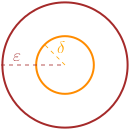
\includegraphics[width=260px]{../figures/balls.svg}
\end{center}

The definition compares two balls centered at the equilibrium.

\begin{itemize}
\item an outer ball of radius $\varepsilon$
\item a smaller ball of radius $\delta$
\end{itemize}

The outer ball represents how far we allow the trajectory to move
from the equilibrium.  
The inner ball represents how close the initial condition must be.

The definition requires that trajectories starting inside the
$\delta$ ball remain inside the $\varepsilon$ ball for all future time.

\textbf{Lyapunov stability}

\begin{center}
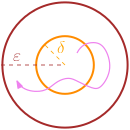
\includegraphics[width=260px]{../figures/lyap.svg}
\end{center}

Trajectories starting in the $\delta$ neighborhood may move away
from the origin and even leave the $\delta$ ball.

However, they remain confined inside the larger $\varepsilon$ ball.
The state never escapes the neighborhood of the equilibrium.

Thus Lyapunov stability is a property of \emph{confinement}.

The definition does not require trajectories to converge to the
equilibrium. They may continue moving indefinitely inside the
$\varepsilon$ region.

\textbf{Instability}

\begin{center}
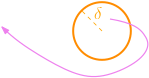
\includegraphics[width=260px]{../figures/unstable.svg}
\end{center}

An equilibrium is unstable if arbitrarily small perturbations can
eventually move away from it.

Even if the initial state starts extremely close to the equilibrium,
the trajectory may leave any prescribed neighborhood.

\textbf{Asymptotic stability}

\begin{center}
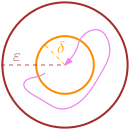
\includegraphics[width=260px]{../figures/asymp.svg}
\end{center}

A stronger notion of stability occurs when trajectories not only
remain close to the equilibrium but also converge to it:

\[
\lim_{t\to\infty} x(t) = 0 .
\]

In this case the equilibrium is called \textbf{asymptotically stable}.

\textbf{The role of the quantifiers}

The order

\[
\forall \varepsilon > 0 \quad \exists \delta(\varepsilon) > 0
\]

is essential.

First the size of the allowed neighborhood $\varepsilon$ is chosen.
Then we must determine how small the initial perturbation $\delta$
must be so that trajectories never leave that neighborhood.

Smaller values of $\varepsilon$ typically require smaller values of
$\delta$.
